\section{Methodology}

\begin{frame}{Flow of MAB Based CMA-ES}
  \includegraphics[bb= 77 150 642 546, clip, width = .9\textwidth]{FlowMAB.eps}
\end{frame}
%\begin{frame}{Clustering}
%  \begin{itemize}
%    \item In this work we adopt $k$-means for dividing.
%        \begin{itemize}
%          \item An effective vector-quantization approach
%          \item Categorizing initial population into $k$ groups
%        \end{itemize}
%    \end{itemize}
%    \begin{columns}
%      \begin{column}{0.2\textwidth}
%        \begin{figure}
%          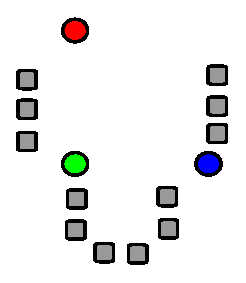
\includegraphics[width=.8\textwidth]{K_Means_Example_Step_1.eps}
%        \end{figure}
%        
%      \end{column}
%      \begin{column}{0.2\textwidth}
%        \begin{figure}
%          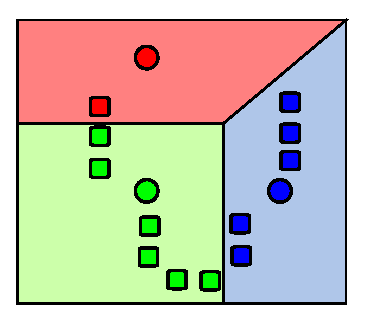
\includegraphics[width=.8\textwidth]{K_Means_Example_Step_2.eps}
%        \end{figure}
%        
%      \end{column}
%      \begin{column}{0.2\textwidth}
%        \begin{figure}
%          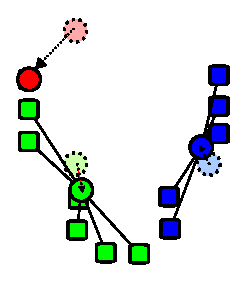
\includegraphics[width=.8\textwidth]{K_Means_Example_Step_3.eps}
%        \end{figure}
%        
%      \end{column}
%      \begin{column}{0.2\textwidth}
%        \begin{figure}
%          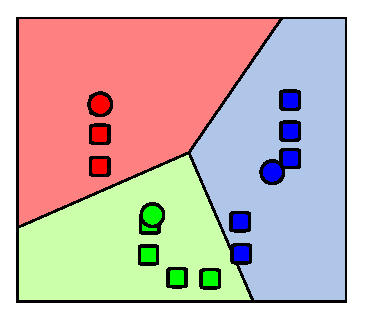
\includegraphics[width=.8\textwidth]{K_Means_Example_Step_4.eps}
%        \end{figure}
%        
%      \end{column}
%    \end{columns}
%
%\end{frame}

\begin{frame}{Multi-armed Bandit problem}
  \begin{itemize}
    \item Investigate the trade-off between exploration and exploitation
      to maximize reward in limit times
      \vspace*{14pt}
    \item Upper Confidence Bound (UCB)
      \vspace*{14pt}
    \item Each time UCB1-tuned selects machine $j$ that maximizes
\[\bar{x_j} + \sqrt{\frac{\ln{n}}{n_j}
          \min(\frac{1}{4},V_j(n_j))}\], where $V_j(t) =\sigma_j^2 +
          \sqrt{\frac{2\ln n}{n_j}}$.

      \begin{itemize}
        \item $\bar{x_j}$: the average reward of machine $j$.
        \item $n_j$: the number of times machine $j$ has been played.
        \item $n$: the played times of overall system.
      \end{itemize} 
  \end{itemize}
\end{frame}

%\begin{frame}{Multi-armed Bandit Problem}
%  \begin{itemize}
%    \item Investigate the trade-off between exploration and exploitation
%      \vspace*{10pt}
%    \item Assume there are $k$ independent slot machines
%      \vspace*{10pt}
%    \item Each machine generates reward according to its own unknown probability
%      distribution.
%      \vspace*{10pt}
%    \item We can only observe the playing sequence and the correlated
%      reward.
%      \vspace*{10pt}
%    \item The goal is to maximize reward in limited play times.
%      \vspace*{10pt}
%  \end{itemize}
%  \begin{figure}
%    \flushright
%    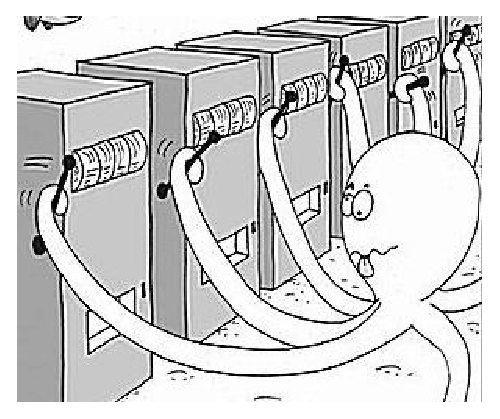
\includegraphics[width = 0.3\textwidth]{MAB-2.eps}
%  \end{figure}
%\end{frame}
%
%\begin{frame}{Upper Confidence Bound }
%  \begin{itemize}
%    \item A family of solutions to MAB problems
%      \vspace*{14pt}
%    \item UCB1 -- the first Upper Confidence Bound (UCB) algorithm
%      \vspace*{14pt}
%    \item Play machine $j$ which maximizes
%      \[\bar{x_j} + \sqrt{\frac{2\ln n}{n_j}}\]
%      \begin{itemize}
%        \item $\bar{x_j}$: the average reward of machine $j$.
%        \item $n_j$: the number of times machine $j$ has been played.
%        \item $n$: the played times of overall system.
%      \end{itemize} 
%  \end{itemize}
%\end{frame}
%
%\begin{frame}{UCB1-tuned}
%  \begin{itemize}
%    \item UCB1 takes no variance into consider.
%      \begin{itemize}
%        \item UCB1-tuned is the version which adds variance as a factor.
%        \item UCB1-tuned is not proven working well but outperforms UCB1 in
%          practice.
%        \item In UCB1-tuned, the machine $j$ to be played is with the
%          highest \[\bar{x_j} + \sqrt{\frac{\ln{n}}{n_j}
%          \min(\frac{1}{4},V_j(n_j))}\], where $V_j(t) =\sigma_j^2 +
%          \sqrt{\frac{2\ln n}{n_j}}$.
%      \end{itemize}
%      \vspace*{14pt}
%    \item UCB1-tuned is adopted in our work.
%  \end{itemize}
%
%\end{frame}

\begin{frame}{Replacement Strategy} 
\begin{itemize} 
  \item By generating a new arm and sampling from the distribution of
          that arm, we can replace the worst arm by the newly generated
          one.  
          \vspace*{14pt}
    \item There are 2 judgement to distinguish if there is any arm to
      be replaced.
      \begin{enumerate}
        \item If an arm samples no better solution in a period of time.
        \item If an arm has not been pulled for a long while.
      \end{enumerate}
  \end{itemize}
\end{frame}
\begin{frame}{Implementation of Proposed System}
  Here we give a simple description about our system.
  \vspace*{8pt}
  \only<1>{
  \begin{figure}
    \includegraphics[scale = 0.4]{animation1.eps}
  \end{figure}
}
  \only<2>{
  \begin{figure}
    \includegraphics[scale = 0.4]{animation2.eps}
  \end{figure}
}
  \only<3>{
  \begin{figure}
    \includegraphics[scale = 0.4]{animation3.eps}
  \end{figure}
}
  \only<4>{
  \begin{figure}
    \includegraphics[scale = 0.4]{animation4.eps}
  \end{figure}
}
  \only<5>{
  \begin{figure}
    \includegraphics[scale = 0.4]{animation5.eps}
  \end{figure}
}
  \only<6>{
  \begin{figure}
    \includegraphics[scale = 0.4]{animation6.eps}
  \end{figure}
}
  \only<7>{
  \begin{figure}
    \includegraphics[scale = 0.4]{animation7.eps}
  \end{figure}
}
  \only<8>{
  \begin{figure}
    \includegraphics[scale = 0.4]{animation8.eps}
  \end{figure}
}
\end{frame}





%\begin{frame}{Flow of Proposed Template}
%  \begin{columns}
%    \begin{column}{0.9\textwidth}
%      \begin{figure}[b]
%        \vspace*{1cm}        
%        \includegraphics[width = 0.6\textwidth]{Flow.eps}\hspace*{2cm}
%        \caption{Flow}
%      \end{figure}
%    \end{column}
%  \end{columns}
%\end{frame}
%
%\begin{frame}
%  \frametitle{Pseudo-code of Template}
%
%  \scalebox{0.8}{%
%    \begin{algorithm}[H]
%      \Begin{
%        Initializing population\;
%        Clustering\;
%        \While{not terminate}{
%          \While{any group has not been evolved for certain generation}{
%            Evolving each group\;
%          }
%          Selecting candidates for each group\;
%          Evolving the selected solutions\;
%        } 
%      }
%      \TitleOfAlgo{Overview for the system}
%    \end{algorithm}
%  }
%\end{frame}   
%
%\begin{frame}{Undetermined Components}
%  \begin{itemize}
%    \item The method for making division
%      \vspace*{14pt}
%    \item The criterion of selecting representative solutions for
%      each group
%      \vspace*{14pt}
%    \item The method for evolving the selected candidates
%  \end{itemize}
%\end{frame}
%
%\begin{frame}{Making Division}
%  \begin{itemize}
%    \item The initial population is expected to categorized according to position.
%      \begin{itemize}
%        \item Roughly expresses the diversity
%        \item A population in a specific region is expected driven
%          toward the identical local optimum.
%        \item In other words, a group can be roughly viewed as points
%          near by one specific valley. 
%      \end{itemize}
%      \vspace*{14pt}
%    \item Space locality plays an important role.
%      \begin{itemize}
%        \item Applying clustering
%      \end{itemize}
%  \end{itemize}
%\end{frame}
%
%\begin{frame}{\emph{k-means}}
%  \begin{itemize}
%    \item \emph{k-means} clustering is a basic method for vector quantization.
%      \begin{itemize}
%        \item Partitioning $n$ solutions into $k$ mutual independent
%          clusters.
%        \item Serving as a prototype
%      \end{itemize}
%      \vspace*{14pt}
%    \item Number of clusters
%      \begin{itemize}
%        \item As known as number of groups.
%        \item Without $k$, finding optimal is said to be NP-hard.  
%        \item To define a proper $k$ is difficult.
%      \end{itemize}
%      \vspace*{14pt}
%    \item  Heuristic algorithms for approximation.
%      \begin{itemize}
%        \item Forgy method for initialization
%        \item iteratively refinements until convergence
%      \end{itemize}
%
%  \end{itemize}
%\end{frame}
%
%\begin{frame}{Algorithm of Approximation to k-means}
%
%  \scalebox{0.8}{%  
%    \begin{algorithm}[H]
%      \label{algo:kmeans}
%      \KwIn{$k$, $d$, $\{o_1, o_2,\ldots, o_n\}$ as observations} 
%      \KwOut{$\mathcal{S}$} 
%      Initial: $m_1, m_2,\ldots, m_k$ are
%      random selected from observations as initial centers 
%      \tcp*{Forgy method}
%      \While{At least one of the observations moves to other group} 
%      {\For{j = 1 to k} 
%      {$S_j = \emptyset$  \;} 
%      \For{i = 1 to n} {assign $o_i$ to $S_j$ if $o_i$ is
%      closest to $m_j$ among the $k$ centers\;} 
%      \For{j = 1 to k} {$m_j$ is updated by the arithmetic mean of all vectors $\in S_j$\;}
%    }
%    \TitleOfAlgo{Clustering heuristic function}
%  \end{algorithm}
%}
%
%\end{frame}
%
%\begin{frame}{Illustration for The Algorithm}
%  \begin{columns}
%
%    \begin{column}{0.23\textwidth}
%      \begin{figure}[h]
%        \centering
%        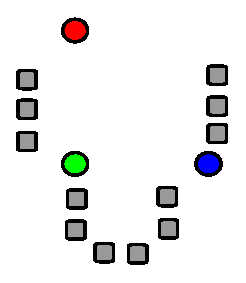
\includegraphics[scale = 0.5]{K_Means_Example_Step_1.eps}
%      \end{figure}
%    \end{column}
%
%    \begin{column}{0.23\textwidth}
%      \begin{figure}[h]
%        \centering
%        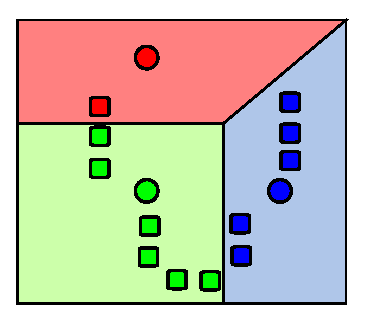
\includegraphics[scale = 0.5]{K_Means_Example_Step_2.eps}
%      \end{figure}
%    \end{column}
%
%    \begin{column}{0.23\textwidth}
%      \begin{figure}[h]
%        \centering
%        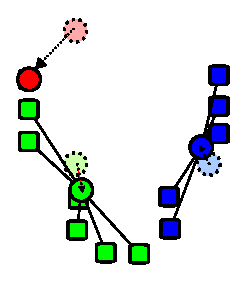
\includegraphics[scale=0.5]{K_Means_Example_Step_3.eps}
%      \end{figure}
%    \end{column}
%
%    \begin{column}{0.23\textwidth}
%      \begin{figure}[h]
%        \centering
%        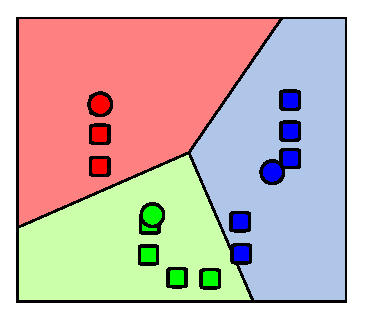
\includegraphics[scale = 0.5]{K_Means_Example_Step_4.eps}
%      \end{figure}
%    \end{column}
%  \end{columns}
%\end{frame}
%
%\begin{frame}{Remaining Criteria}
%  \begin{itemize}
%    \item How to select representativeness from each group?
%      \begin{itemize}
%        \item Using the optimal solution found so far as the representativeness in
%          each group
%      \end{itemize}
%      \vspace*{14pt}
%    \item How to evolve selected candidates?
%      \begin{itemize}
%        \item Evolving them with CMA-ES
%        \item The so-called `outer CMA-ES'
%        \item Aims to observe if better regions can be reached
%      \end{itemize}
%      \vspace*{14pt}
%    \item The number of solutions in a group is fixed after clustering.
%      \begin{itemize}
%        \item Once a better solution is generated, the worst one should
%          be replaced.
%      \end{itemize}
%  \end{itemize}
%\end{frame}
%
%\begin{frame}{An Implementation of the Template}
%  \scalebox{0.8}
%  {
%    \begin{algorithm}[H]{
%        \KwIn{$n$,$t$}
%        \KwOut{best solution ever evolved}
%        Uniformly sampled population of size $n$\;
%        $k = \sqrt{\frac{n}{2}}$\;
%        Integrating \emph{k-means} with \emph{Frogy-method} to cluster the
%        $n$ individuals into $k$ groups\;
%
%        $C\leftarrow$ array with size $k$\;
%        \For{i = 1 to k}
%        {
%          Optimizing group$_i$ by adopting CMA-ES for $t$ generations\;
%          $C_i\leftarrow$ best solution\;
%          Applying CMA-ES to evolve the population consisting of local
%          optima of groups, as known as $C$, until terminated.\;
%        }
%      }
%      \TitleOfAlgo{2-layer CMA-ES}
%    \end{algorithm} 
%  }
%\end{frame}
%
%\begin{frame}
%  \begin{itemize}
%    \item 2-layer CMA-ES addresses the diversity for the search.
%      \vspace*{14pt}
%    \item Next we lay emphasis on finding more promising regions.
%  \end{itemize}
%
%\end{frame}
%
%\begin{frame}{Exploring}
%  \begin{itemize}
%    \item Based on current groups, we aim to figure out better
%      solutions.
%      \begin{itemize}
%        \item According to our hypothesis, the implicit information is
%          hidden between groups.
%        \item What is a good way to evolve groups?
%      \end{itemize}
%      \vspace*{14pt}
%    \item We consider the priority
%      \begin{itemize}
%        \item Put less concentration on groups which performs badly
%        \item Lay emphasis on possible regions
%        \item Without any prior knowledge, a selection strategy is
%          demanded.
%      \end{itemize}
%      \vspace*{14pt}
%    \item The ability to generate new groups adaptively 
%      \begin{itemize}
%        \item We assume a fixed number of groups.
%        \item A replacement strategy is demanded accordingly.
%      \end{itemize}
%  \end{itemize}
%\end{frame}
%
%\begin{frame}{The Selection Strategy}
%
%  \begin{itemize}
%    \item The selection strategy is with the feature that
%      \begin{itemize}
%        \item Given a set of groups, the performance of each group is
%          evaluated through trials
%        \item Lays emphasis on better performance groups
%        \item groups with worse performance would not be ignored
%          permanently
%      \end{itemize}
%      \vspace*{14pt}
%    \item This is just identical to the Multi-armed Bandit (MAB)
%      problem.
%  \end{itemize}
%\end{frame}
%
%
%
%
%\begin{frame}{Flow of MAB-based CMA-ES}
%  \begin{figure}[h]
%    \vspace{15mm}\includegraphics[scale=0.4]{FlowMAB.eps}\hspace{25mm}
%  \end{figure}
%\end{frame}
%
%\begin{frame}{Procedure of MAB-based CMA-ES}
%  \scalebox{0.7}{
%    \begin{algorithm}[H] 
%      \TitleOfAlgo{MAB-based CMA-ES} 
%      \KwIn{$n$,$t$ as a proper generation for each pulling action}
%      \KwOut{best solution ever evolved} 
%      Uniformly sampled population of size $n$\; 
%      $k = \sqrt{\frac{n}{2}}$\; 
%      Integrating \emph{k-means} with \emph{Frogy-method} to cluster the $n$ individuals into
%      $k$  groups as known as bandits\; 
%      $C\leftarrow$ array with size $k$\;
%      \For{i = 1 to k}            
%      { pull($i$)\; $C_i\leftarrow$ best
%      solution\; } 
%      \While{not terminated} 
%      { \For{i = 1 to k} {
%        calculateUCB($i$) \tcp*[r]{calculate modified UCB1-tuned as
%        illustrated above} record the index with max value in $M$\;
%
%      } 
%      pull($M$)\;      
%      $C_M \leftarrow$ best solution in
%    group$_M$\; update()\; }
%  \end{algorithm}  }
%\end{frame}
%
%\begin{frame}
%  \scalebox{0.65}{
%    \begin{algorithm}[H]
%      Initial $P\leftarrow $ a permutation array from $1$ to $k$\; 
%      ToBeDeleted = $0$\;
%      \For{i = 1 to k} 
%      {
%        \If{deleting criterion 1 is met in group$_{P_i}$} 
%        {
%          ToBeDeleted = $P_i$\; 
%        }  
%
%      }
%      \If{ToBeDeleted = 0} 
%      {
%        \For{i = 1 to k} 
%        {
%          \If{deleting criterion 2 is met in group$_{P_i}$}
%          {
%            ToBeDeleted = $P_i$\;
%          } 
%        } 
%      } 
%      \If{ToBeDeleted = 0} 
%      { 
%        return\; 
%      } 
%      \Else
%      { 
%        $s\leftarrow$ ToBeDeleted\; 
%        generate a new solution as a new group  denoted as $group^\star$ according to $C_1, C_2,\ldots, C_{s_{i-1}}, C_{s_{i+1}},\ldots, C_k$ \; 
%        \For{i = 1 to $\|group_{s}\|-1$} 
%        { pull($group^\star$) without replacing worst\; }
%        replace $group_{s}$ with $group^\star$\; return\; 
%      } 
%      \TitleOfAlgo{update}
%    \end{algorithm} 
%  }
%\end{frame}
